%!TEX root = ../main.tex

\section{More Divide and Conquer}

\subsection{Polynomial Multiplication}

The problem we will solve will be to multiply two polynomials.
Let $A = a_dx^d + a_{d-1}x^{d-1} + ... + a_1x + a_0$, and let
$B = b_dx^d + b_{d-1}x^{d-1} + ... + b_1x + b_0$. In high school we
would multiply $A$ and $B$ as $C = A \cdot B$ with

$$
C = \underbrace{a_db_dx^{2d} + a_db_{d-1}x^{2d-1} + ... + a_db_0x^d}_{
    \text{first term in the product}
} + \; ...
$$

This technique has an upper bound of $O(n^2)$ however. We want to beat
this algorithm using divide and conquer.

\begin{remark}
    One can use this technique to multiply integers. Just set
    $x = 10$ and let $a_i$ be the $i$-th digit of the integer.
\end{remark}

\subsubsection{First Attempt}

Let's assume that the number of coefficients of the polynomials are a
power of 2 (for simplicity). That means $d = 2^k - 1$. We split each
polynomial in half so that each half has 
$\frac{d + 1}{2}$ elements. For instance for $A$ we have that
$A_h' = a_dx^d + ... + a_{\frac{d+1}{2}}x^{\frac{d+1}{2}} $ and
$A_l = a_{\frac{d-1}{2}}x^{\frac{d-1}{2}} + ... + a_1x + a_0$.
Now we have that $A = x^{\frac{d+1}{2}}A_h + A_l$ and similarly
$B = x^{\frac{d+1}{2}}B_h + B_l$. We are now in a position to multiply

\begin{align}
    A \cdot B &= (x^{\frac{d+1}{2}}A_h + A_l) (x^{\frac{d+1}{2}}B_h +
    B_l) \\
    &= A_hB_h + x^{\frac{d+1}{2}}(A_hB_l + A_lB_h) + A_lB_l
\end{align}

Let $T(n)$ be the time taken to multiply two polynomials with $n$
coefficients. Then

$$
T(n) \leq 4T(\frac{n}{2}) + cn \implies T(n) = O(n^2)
$$

Unfortunately, this technique didn't save us time. But we can refine
it in the following manner with a little trick. Notice that 
on (4.2) we want to multiply three products.

\begin{itemize}
    \item $A_hB_h$: we have to multiply this no matter what.
    \item $A_lB_l$: same as above.
    \item $A_hB_l + A_lB_h$: this consists of two products which is
    what is making the above technique have a $O(n^2)$ upper bound.
    Can we somehow multiply only one product? Yes! Notice that
    $$
    (A_h + A_l)(B_h + B_l) = \underbrace{A_hB_h}_{\text{what we have}}
    + \underbrace{A_hB_l + A_lB_h}_{\text{what we want}} +
    \underbrace{A_lB_l}_{\text{what we have}}
    $$
    So then
    $$
    A_hB_l + A_lB_h = (A_h + A_l)(B_h + B_l) - A_hB_h - A_lB_l
    $$
    We've reduced the steps necessary as now we only need one
    multiplication instead of two to find $A_hB_l + A_lB_h$.
\end{itemize}

Using the above, we have that

$$
T(n) \leq 3T(\frac{n}{2}) + kn
$$

and using the Master Theorem with $a = 3$, $b = 2$ and $c = 1$ we
learn that the upper bound is $O(n^{\log_2(3)}) \approx O(n^{1.6})$.

\subsection{Convex Hulls on the Plane}

\begin{definition}
    A set $S \subset \mathbb{R}^n$ is said to be convex if for all
    $x, y \in S$ the line segment joining $x$ and $y$ is contained in
    $S$.
\end{definition}

\begin{figure}[hpt]
\centering
\begin{subfigure}{.5\textwidth}
  \centering
  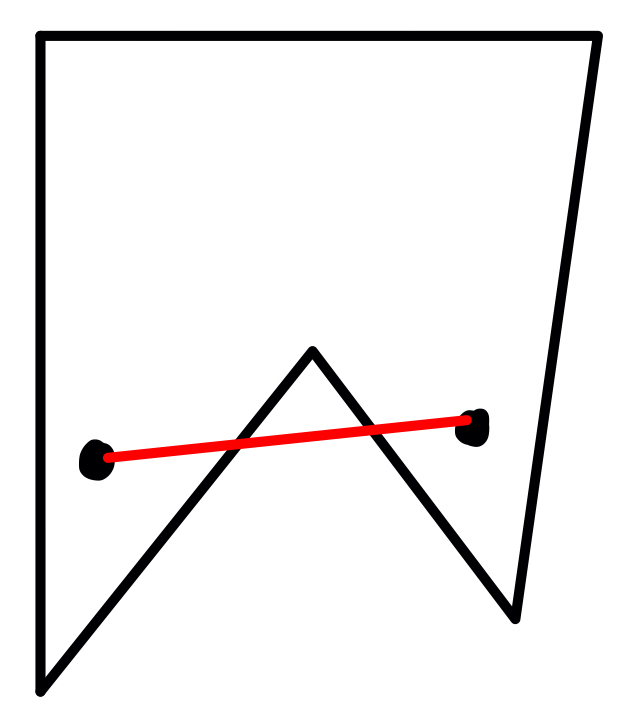
\includegraphics[width=.4\linewidth]{figures/convex-hull-false}
  \caption{Non convex set}
  \label{fig:convex-1}
\end{subfigure}%
\begin{subfigure}{.5\textwidth}
  \centering
  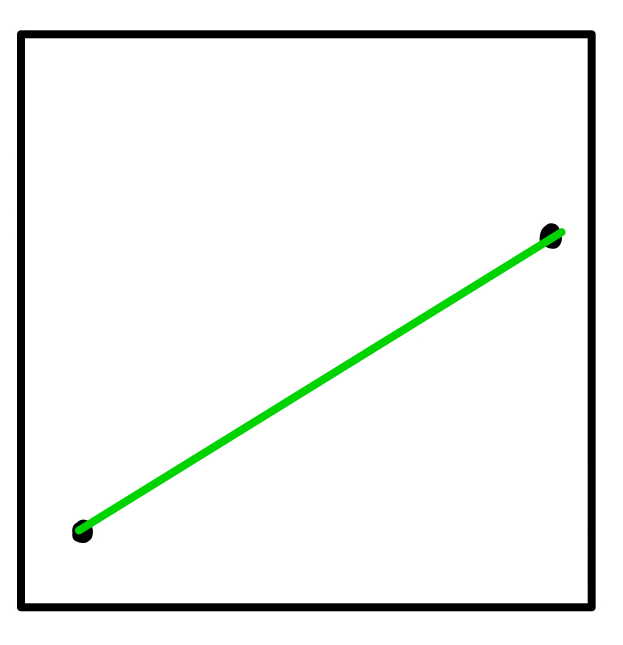
\includegraphics[width=.4\linewidth]{figures/convex-hull-true}
  \caption{Convex set}
  \label{fig:sub2}
\end{subfigure}
\caption{Examples of convex sets}
\label{fig:test}
\end{figure}


\begin{definition}
    Given two points $x = (x_1, x_2)$ and $y = (y_1, y_2)$, the
    convex combination of $x$ and $y$ is defined by
    $$
    \lambda x + (1 - \lambda)y
    $$
    for some $\lambda \in [0, 1]$.
\end{definition}

The convex combination is a way of finding all the points that are in
the line segment of $x$ and $y$.

\begin{definition}
    The convex hull of a finite set of points $S$ is the set of all
    points that can be expressed as convex combinations of points in
    $S$.
\end{definition}

A more pictoral way of defining the convex hull is, given
$S = \{ x_1, ..., x_n \}$, to think of each $x_i$ as a nail, and
we take a rubber band that is originally stretched to infinity, and we
let go of the rubber band. The final position of the rubber band is
the convex hull.

\begin{definition}
    (Another definition of convex hull) The convex hull of a set of
    points is the smallest convex set that
    contains the points.
\end{definition}

\begin{lemma}
    A convex hull is a convex polygon (i.e. no interior angle is
    larger than $\pi$).
\end{lemma}


\subsection{Algorithms to Find the Convex Hull}

Let $(x_1, y_1), ..., (x_n, y_n)$ be the inputs. The output for the
algorithm will be the sequence of points in the boundary in counter
clockwise order.

\subsubsection{Naive Way}

We first produce a simple test: Given a line
by two points and a third point, determine which side of the line the
third point lies on. We claim this is sufficient to find the convex
hull.

To implement this test, suppose we have the line joining $(x_1, y_1)$
and $(x_2, y_2)$ and we consider a point $(x_3, y_3)$. Which side is
this
point on? First, we determine the equation of the line, which is

$$
y - y_1 = \frac{y_2 - y_1}{x_2 - x_1}(x - x_1)
$$

Then we plug in $(x_3, y_3)$ and determine whether $y_3 < mx_3 + b$
or $y_3 > mx_3 + b$ to determine which side of the line the point
lies.

Going back to our naive algorithm:

\begin{itemize}
    \item Take the point $p_k$ with the highest $x$-coordinate. We
    know this
    point must be on the convex hull.
    \item Consider $p_k$ with all other points in $S$.
    \item For each pair $(p_k, p_i)$ check if all the other points lie
    on the same
    side of the line segment joining the pair (use the simple test
    above).
    \item When you find one such pair $(p_k, p_j)$, stop looking for
    more, and repeat this process without considering $p_k$ and
    comparing every other point with $p_j$.
\end{itemize}


This naive algorithm takes $O(n^2)$.


\subsubsection{Divide and Conquer Approach}

\begin{definition}
    A point in one convex hull can \emph{see} a point in another
    convex hull if the segment joining the two points does not
    intersect either hull.
\end{definition}

\begin{definition}
    The upper tangent is the highest line segment joining two points
    on each hull that see each other.
\end{definition}

\begin{definition}
    The lower tangent is the lowest line segment joining two points
    on each hull that see each other.
\end{definition}

\begin{definition}
    We say the line joining point $p$ in hull $C_1$ and point $q$ in
    hull $C_2$ stabs $C_2$ if the continuation of the line goes
    through the interior of $C_2$.
\end{definition}

\begin{remark}
    Recall the simple test above. We can find out when a line stabs
    $C_2$ if the successor of point
    $q$ in $C_2$ is one side of the line and the predecessor of $q$ is
    on the other side of the line.
\end{remark}

The approach for the algorithm is the following:

\begin{itemize}
    \item Divide: Order all points $p_i$ by their $x$-coordinate and
    take the median. Call this point $p_m$. This separates the points
    into two sets, $L$ and $H$.
    \item Conquer: Find the convex hull of $L$ and $H$. The base case
    is when you have three points, which is simply a triangle.
    \item Combine: (Not rigorous at all, mostly shown by picture in
    class) Start by choosing $p$ to be the right-most point in
    the left hull, and $q$ the left-most point in the right hull. Then
    $p$ and $q$ see each other. While the line segment joining these
    two points stabs either $C_1$ or $C_2$, keep "swiveling" these
    until the line segment doesn't stab either hull. You've found the
    upper tangent and lower tangent. This operation takes at most $n$
    for each tangent. Once you've found the upper and lower tangent,
    combine the two hulls as in Figure~\ref{fig:convex-merge}.
\end{itemize}

\begin{figure}[hpt]
    \centering
    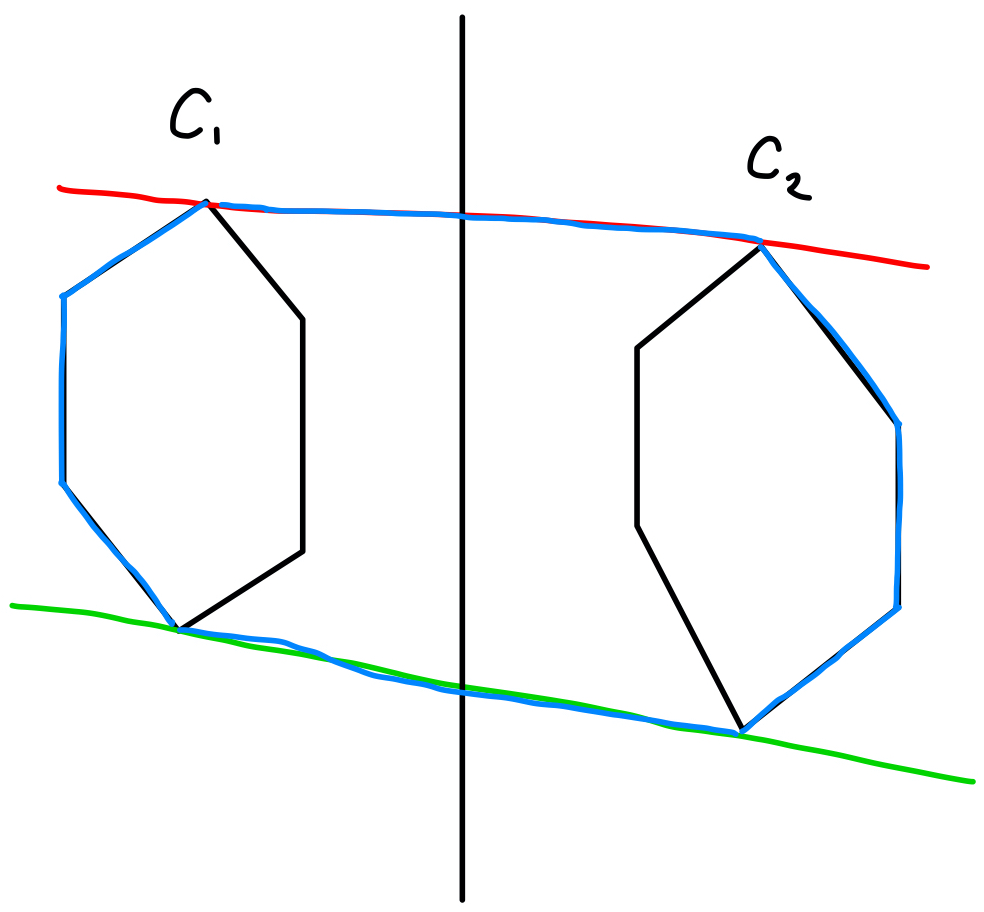
\includegraphics[width=0.4\textwidth]{figures/convex-merge.jpeg}
    \caption{Convex hull combine: In red the upper tangent, in green
    the lower tangent, and in blue the new, merged hull.}
    \label{fig:convex-merge}
\end{figure}






